\chapter{Funktionalität}
\label{chap:funk}
Im Folgenden werden die Funktionalitäten der App hinsichtlich der Anwendernutzung beschrieben. Dabei wird erklärt, wie man Profile anlegt und Daten in ein Profil läd. Zudem werden die Auswertungsseiten der Simulation kurz erläutert. 
	\section{Profilverwaltung}
	\label{sec:profile}
	
	Die Profilverwaltung ist die Startseite der App. Dort können Profile angelegt und gelöscht werden.	
	
	\begin{figure}[H]
		\centering
		\begin{subfigure}[b]{0.45\textwidth}
			\centering
			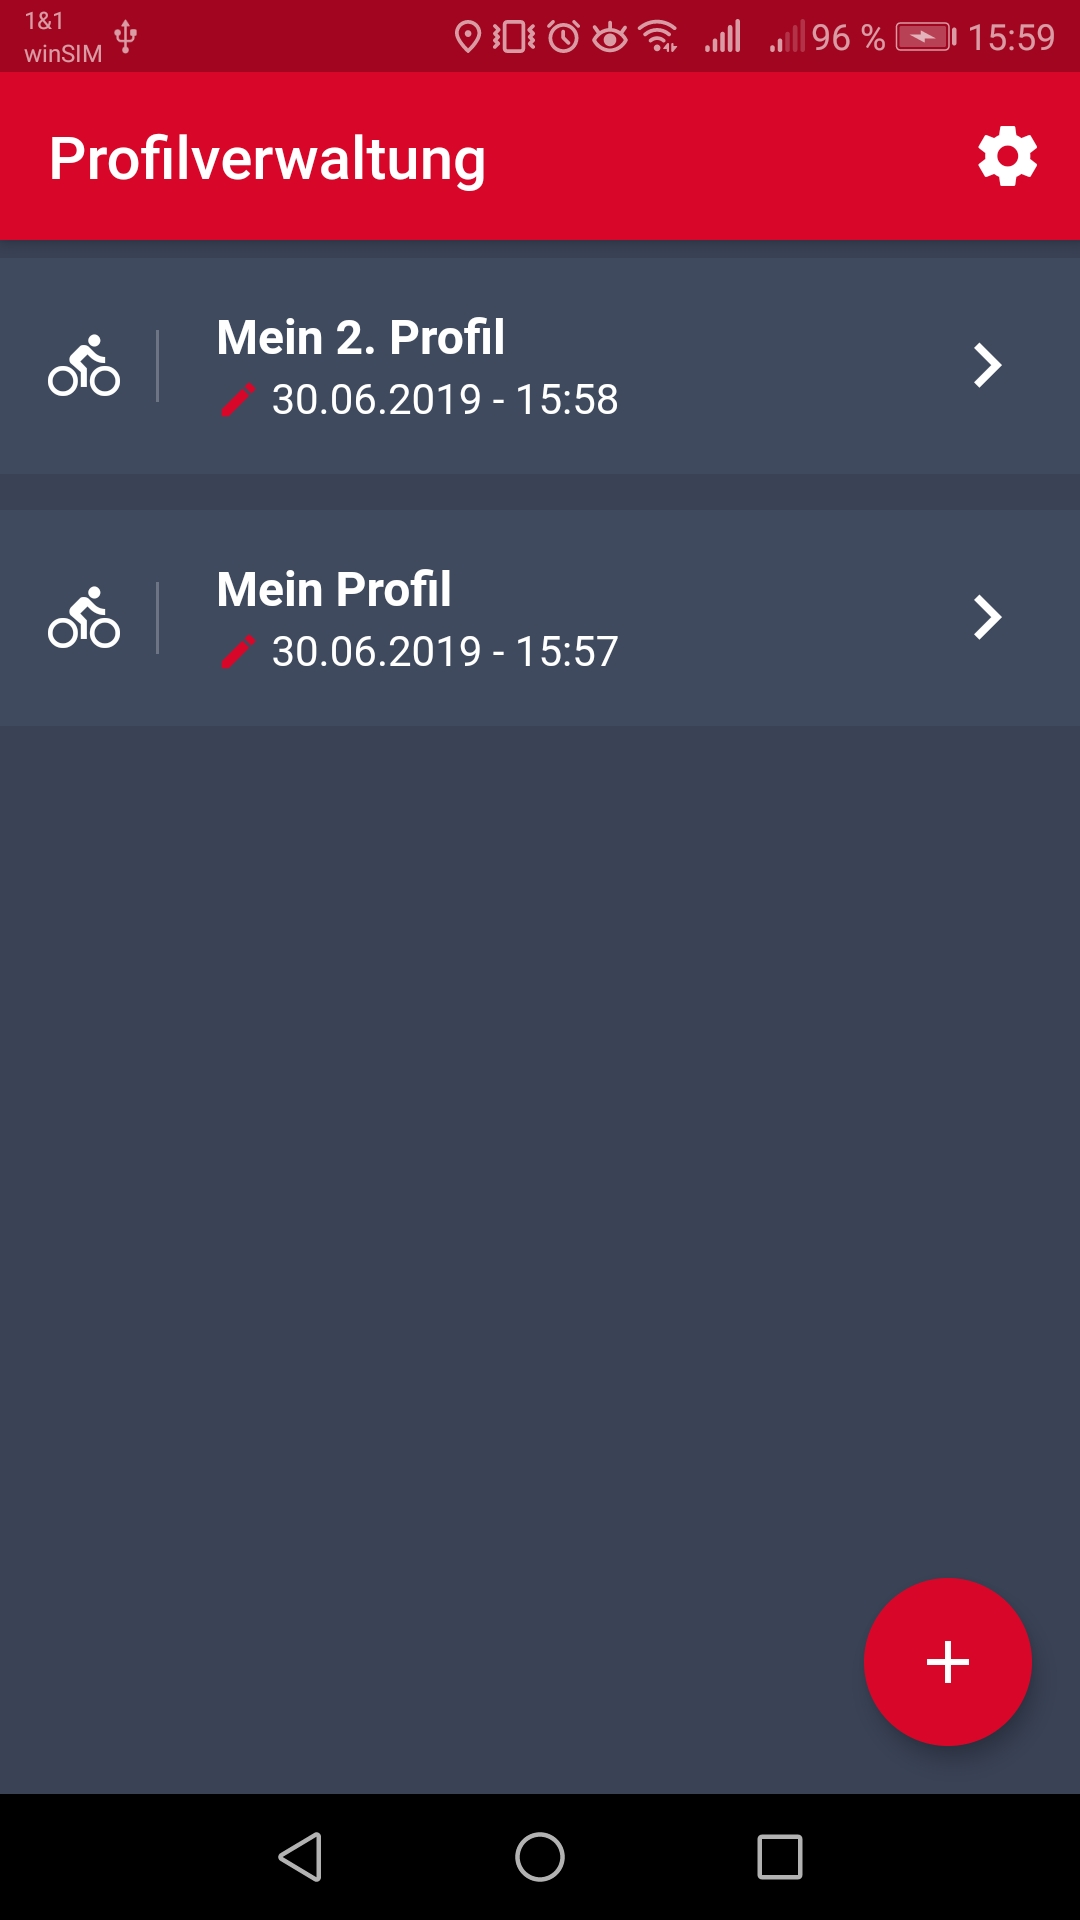
\includegraphics[width=0.85\textwidth]{../include/images/funktionalitaet/profil}
			\label{subfig:profil}
			\subcaption{Profilverwaltung}
		\end{subfigure}
		\hfill
		\begin{subfigure}[b]{0.45\textwidth}
			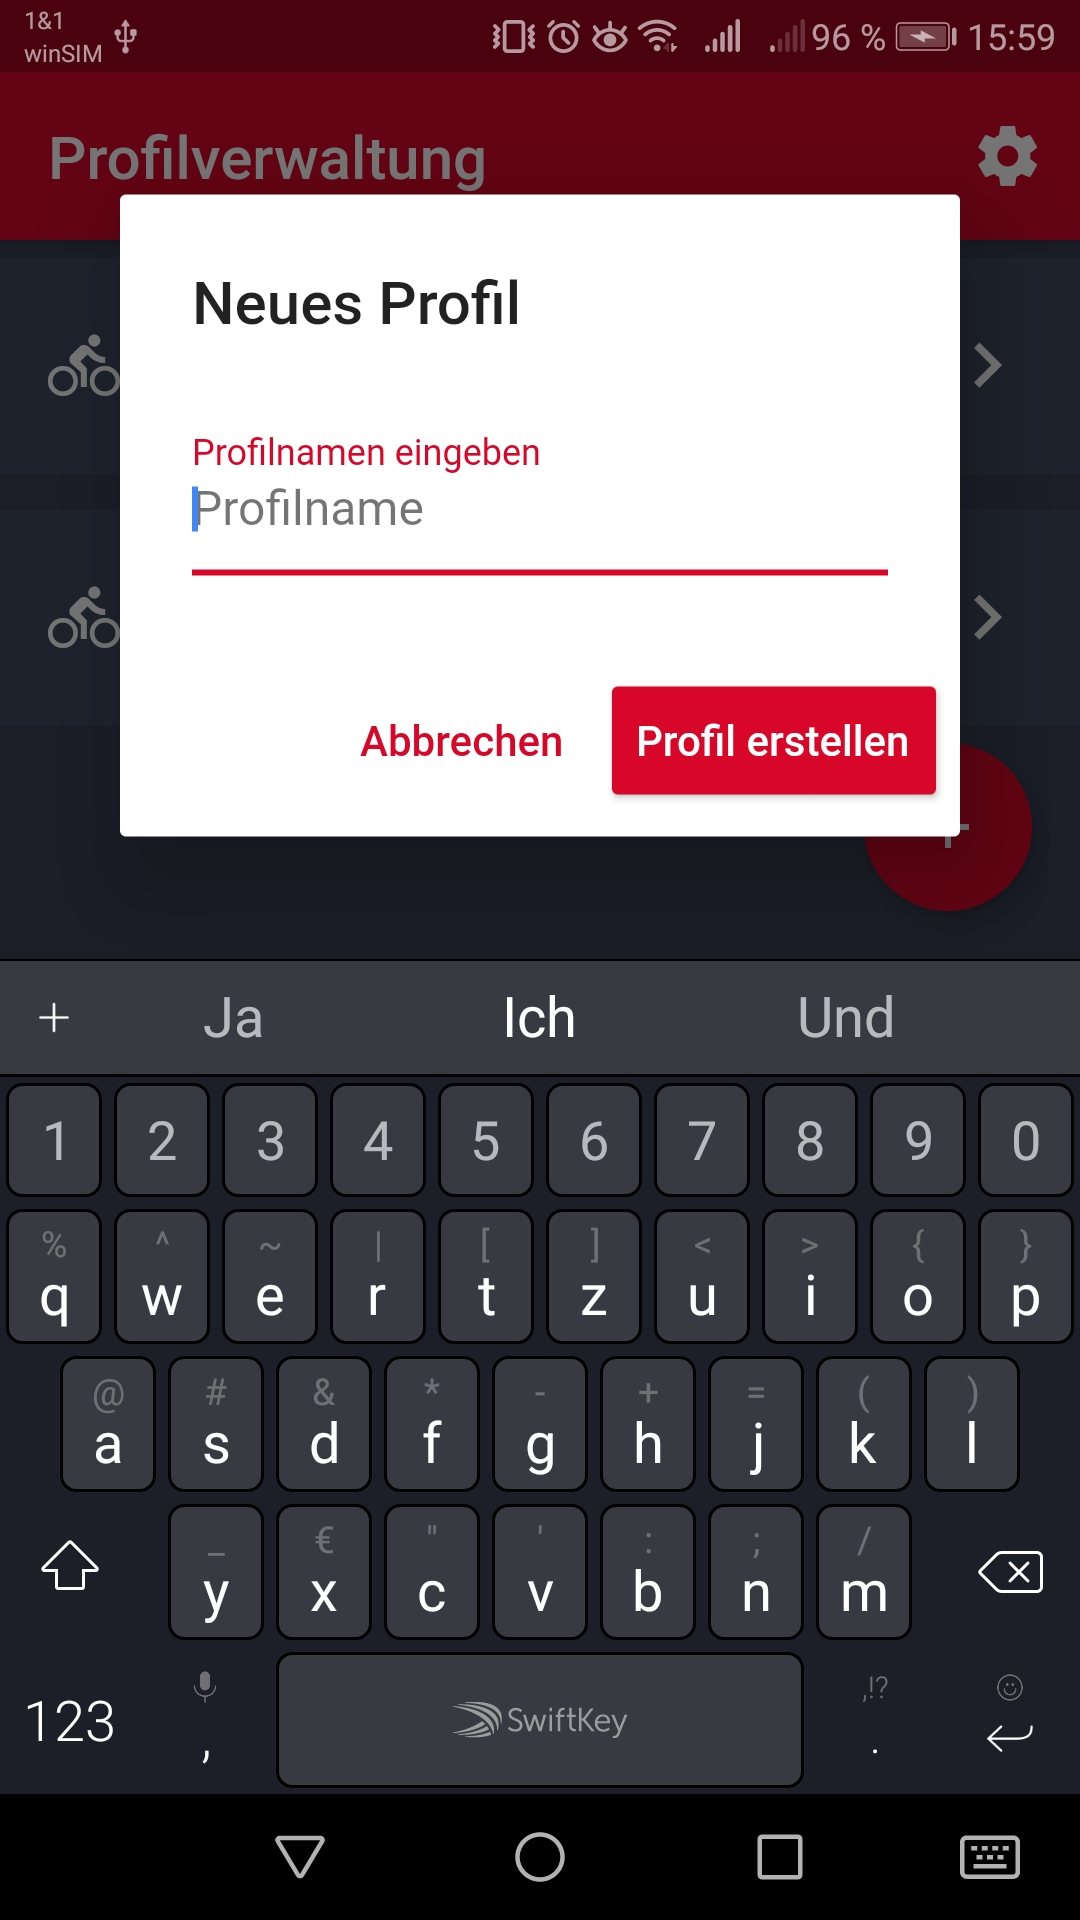
\includegraphics[width=0.85\textwidth]{../include/images/funktionalitaet/profil_eingabe}
			\label{subfig:profil_eingabe}
			\subcaption{ Anlegen eines neuen Profils}
		\end{subfigure}
		\caption{Umsetzung der Profilverwaltung}
		\label{img:settings}
	\end{figure}
	
	\textbf{Anlegen eines Profils}\\
	Das Anlegen eines Profils wird durch Drücken des mit einem \glqq +\grqq{} versehenden Floating-Action-Buttons eingeleitet. Nach drücken des Buttons öffnet sich ein Fenster, wie in \cref{subfig:profil_eingabe} zu sehen. Dort kann über ein Eingabefeld der Profilname hinzugefügt werden. Anschließend kann über den Button \glqq Profil erstellen\grqq{} oder den Button \glqq Abbrechen\grqq{} das hinzufügen eines Profils beendet werden.\\
	
	\textbf{Löschen eines Profils}\\
	Ein Profil kann gelöscht werden indem man eine Wischbewegung (Swipen) nach links auf dem entsprechenden Profil ausführt. Beginnt man die Wischbewegung nach links so, wird das Profil zur Seite geschoben und ein Mülleimericon, sowie der Schriftzug \glqq löschen\grqq{} angezeigt, um den Nutzer davon zu unterrichten, dass seine Aktion zur Löschung des Profils führt. Stoppt man die Wischbewegung bevor das Profil ganz aus dem Bildschirm verschwunden ist, so wird das Löschen abgebrochen.
	

	
	\section{Simulationsdaten laden}
	\label{sec:load-sim-data}
	
	Das Laden der Daten für die Simulation wird auf einer eigenen Seite ausgeführt. Sind keine Daten vorhanden, so wird dies angezeigt. Über einen Floating-Action-Button  ist es möglich ein Buttonmenü zu öffnen. Dies erlaubt dem Nutzer, Daten vom Server zu oder aus einem QR-Code zu laden oder Daten für die Simulation zu bearbeiten. Sind keine Daten geladen, so ist die Bearbeitung der Daten für die Simulation auch nicht nutzbar. Sind bereits Daten für dieses Profil geladen worden, so werden sie direkt geladen, da sie mit dem Profil verbunden sind. Die zu geladenen Daten bestehen aus Kennzahlen, die die in einer Liste angezeigt werden.
	
	

	\begin{figure}[H]
	\begin{subfigure}[b]{0.5\textwidth}
	\centering
		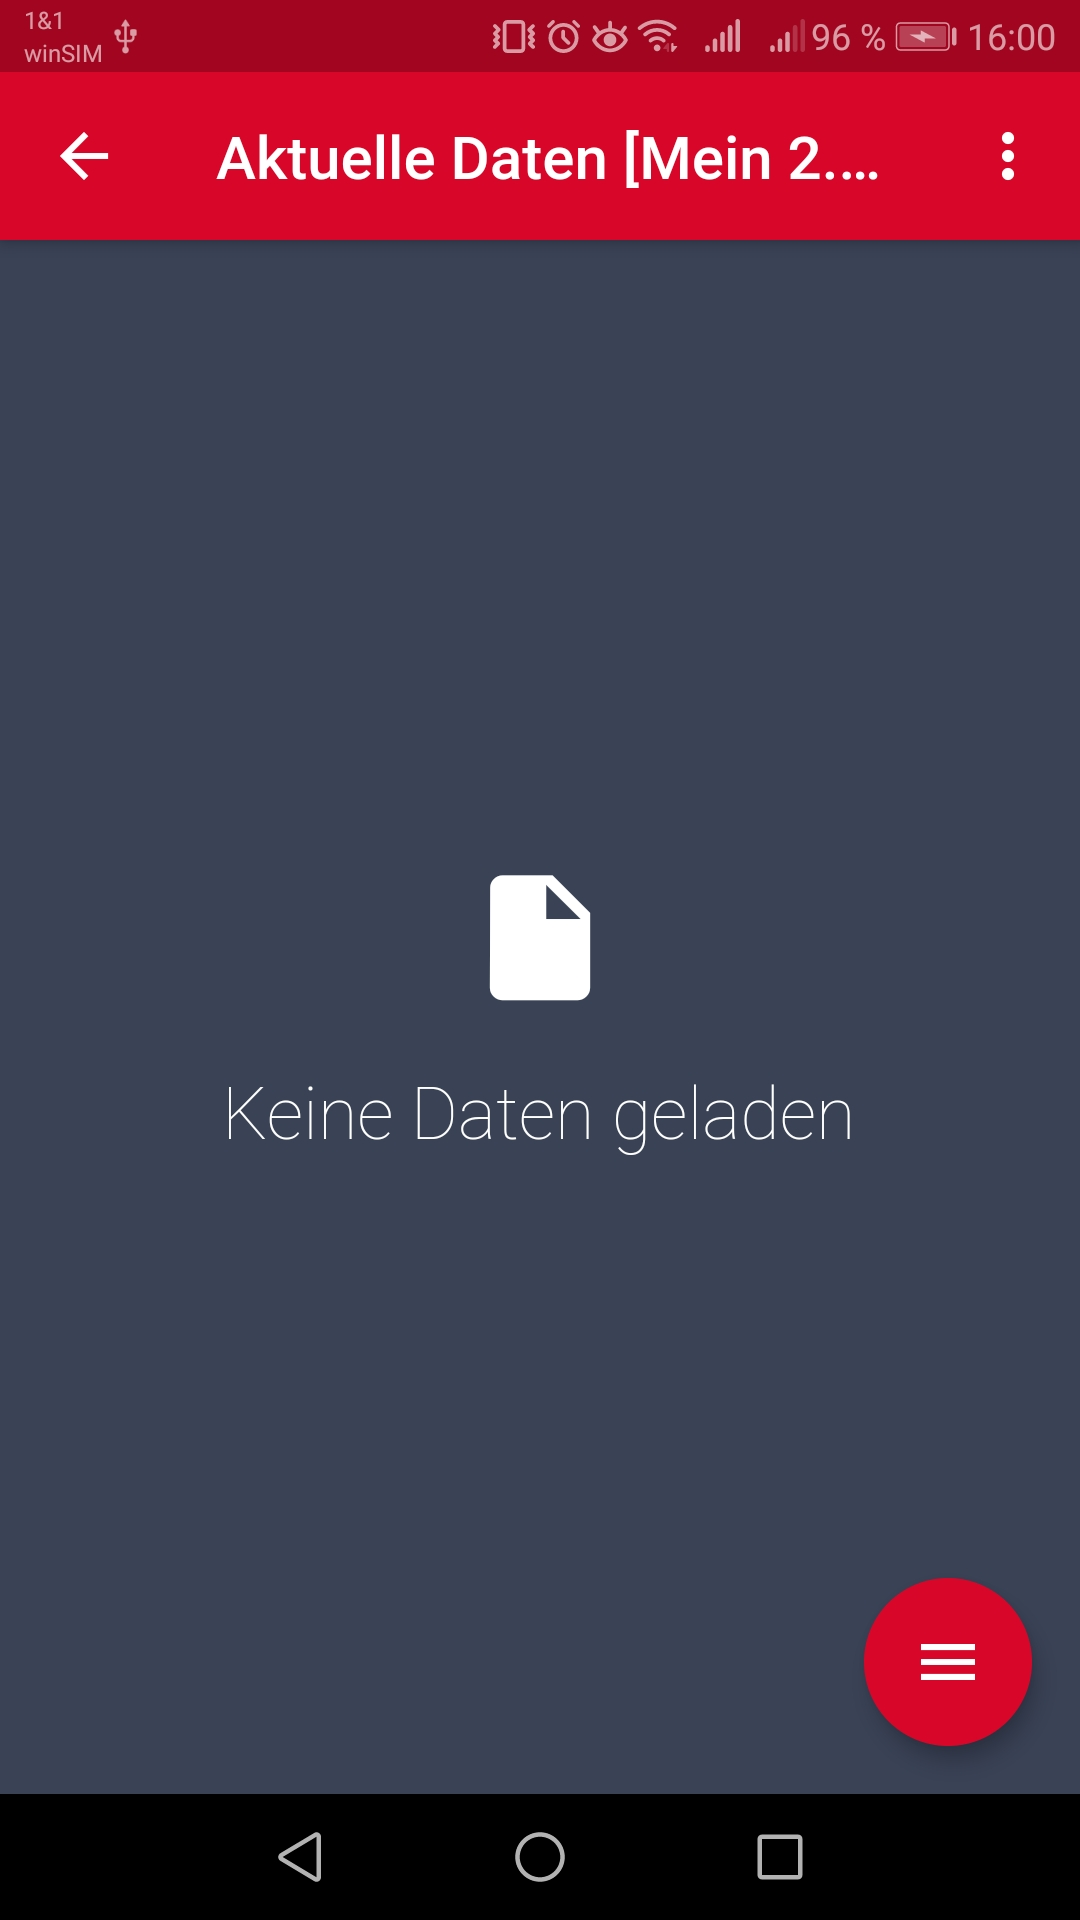
\includegraphics[width=0.6\textwidth]{../include/images/funktionalitaet/dataLaden}
		\subcaption{Seite ohne Daten}
	\end{subfigure}
	\hfill
	\begin{subfigure}[b]{0.5\textwidth}
	\centering
		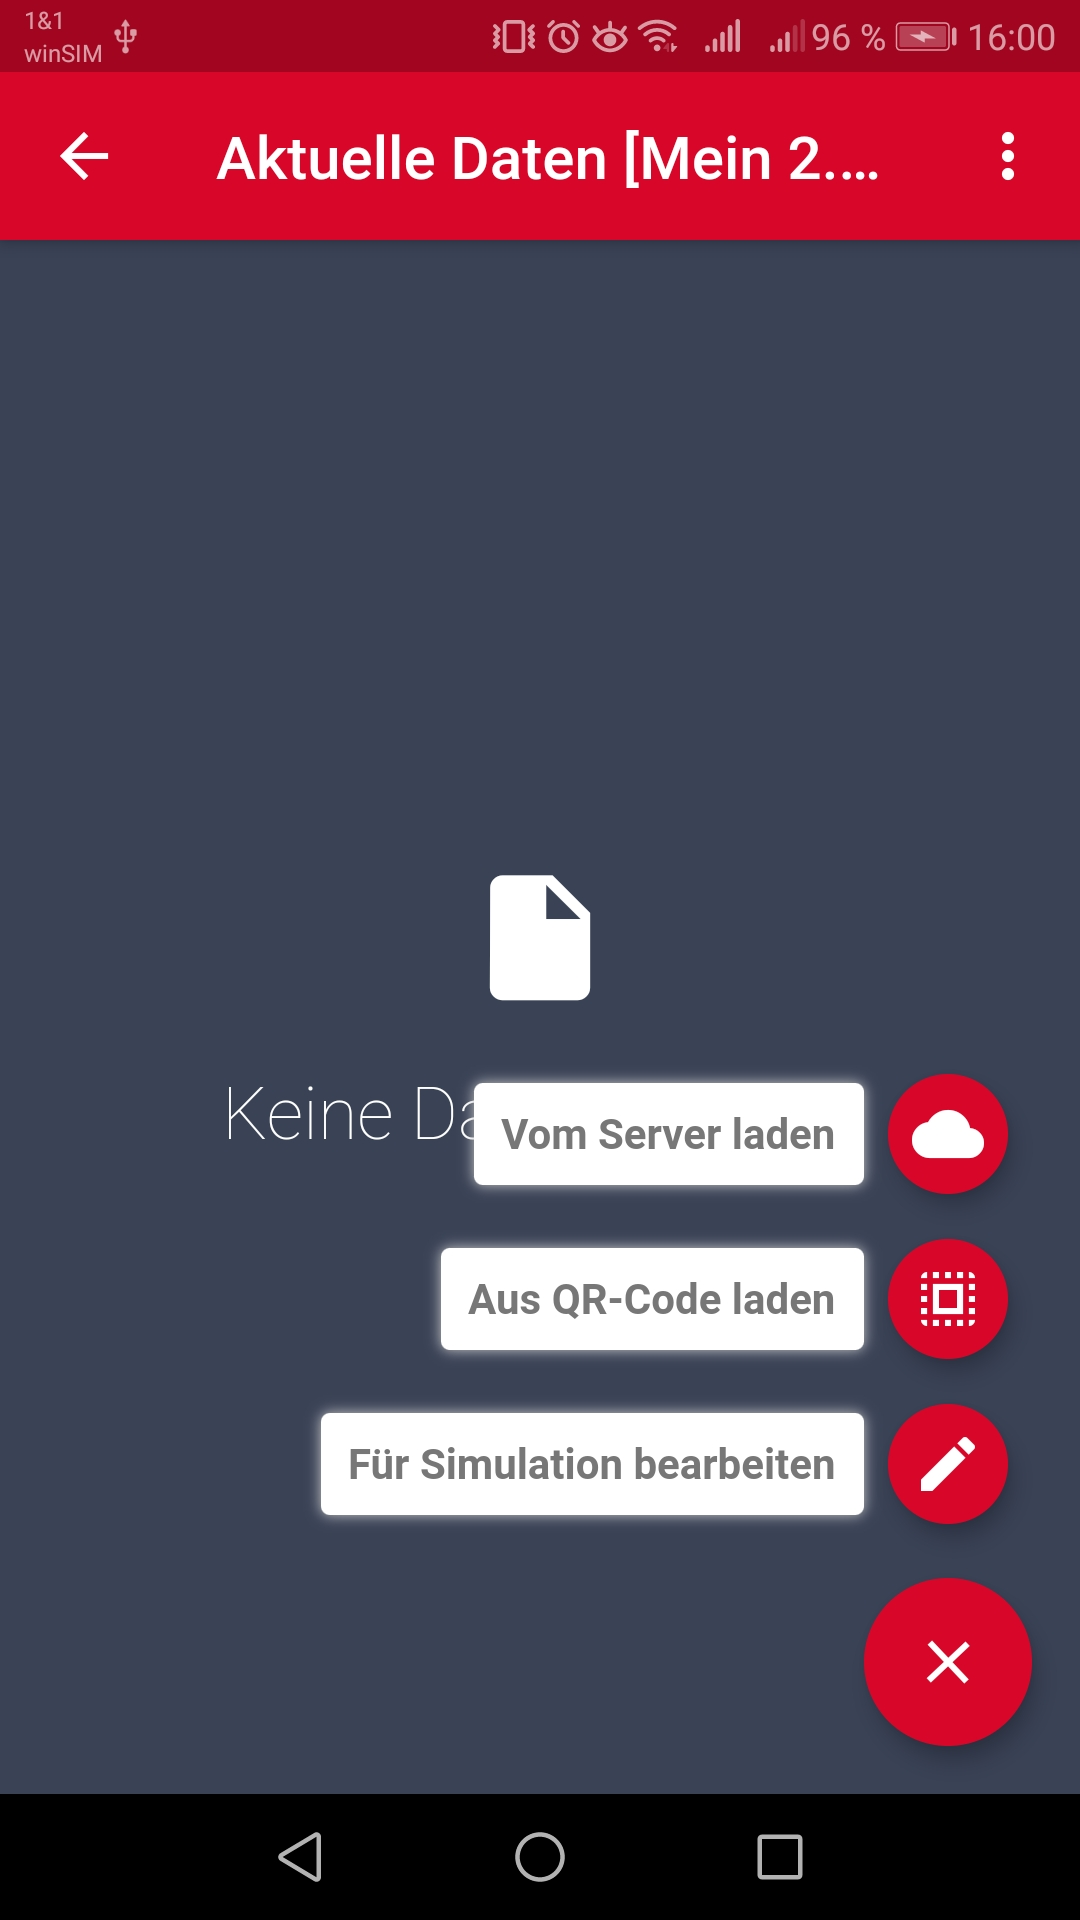
\includegraphics[width=0.6\textwidth]{../include/images/funktionalitaet/dataLaden_buttons}
		\subcaption{Buttonsmenü}
	\end{subfigure}
	
	\caption{Die Laden Daten Ansicht}
\end{figure}

	
		\subsection{Laden vom Server}
		\label{subsec:load-srv}
Drückt man den Button \glqq Vom Server laden\grqq{} so öffnet sich ein Fenster ähnlich zum Anlegen eines neuen Profils. Über ein EIngabefeld muss eine Messungs-ID übergeben werden. Diese bestimmt welche Daten vom Server geladen werden. Durch einen Klick auf \glqq Messung laden \grqq{} oder \glqq Abbrechen \grqq{} kann, die Aktion entsprechend beendet werden. Das Fenster schließt sich und während des Ladens kommt eine kurze Ladeanimation. Sind die Daten geladen, so werden diese nun angezeigt.\\
		
		\begin{figure}[H]
	\begin{subfigure}[b]{0.5\textwidth}
		\centering
		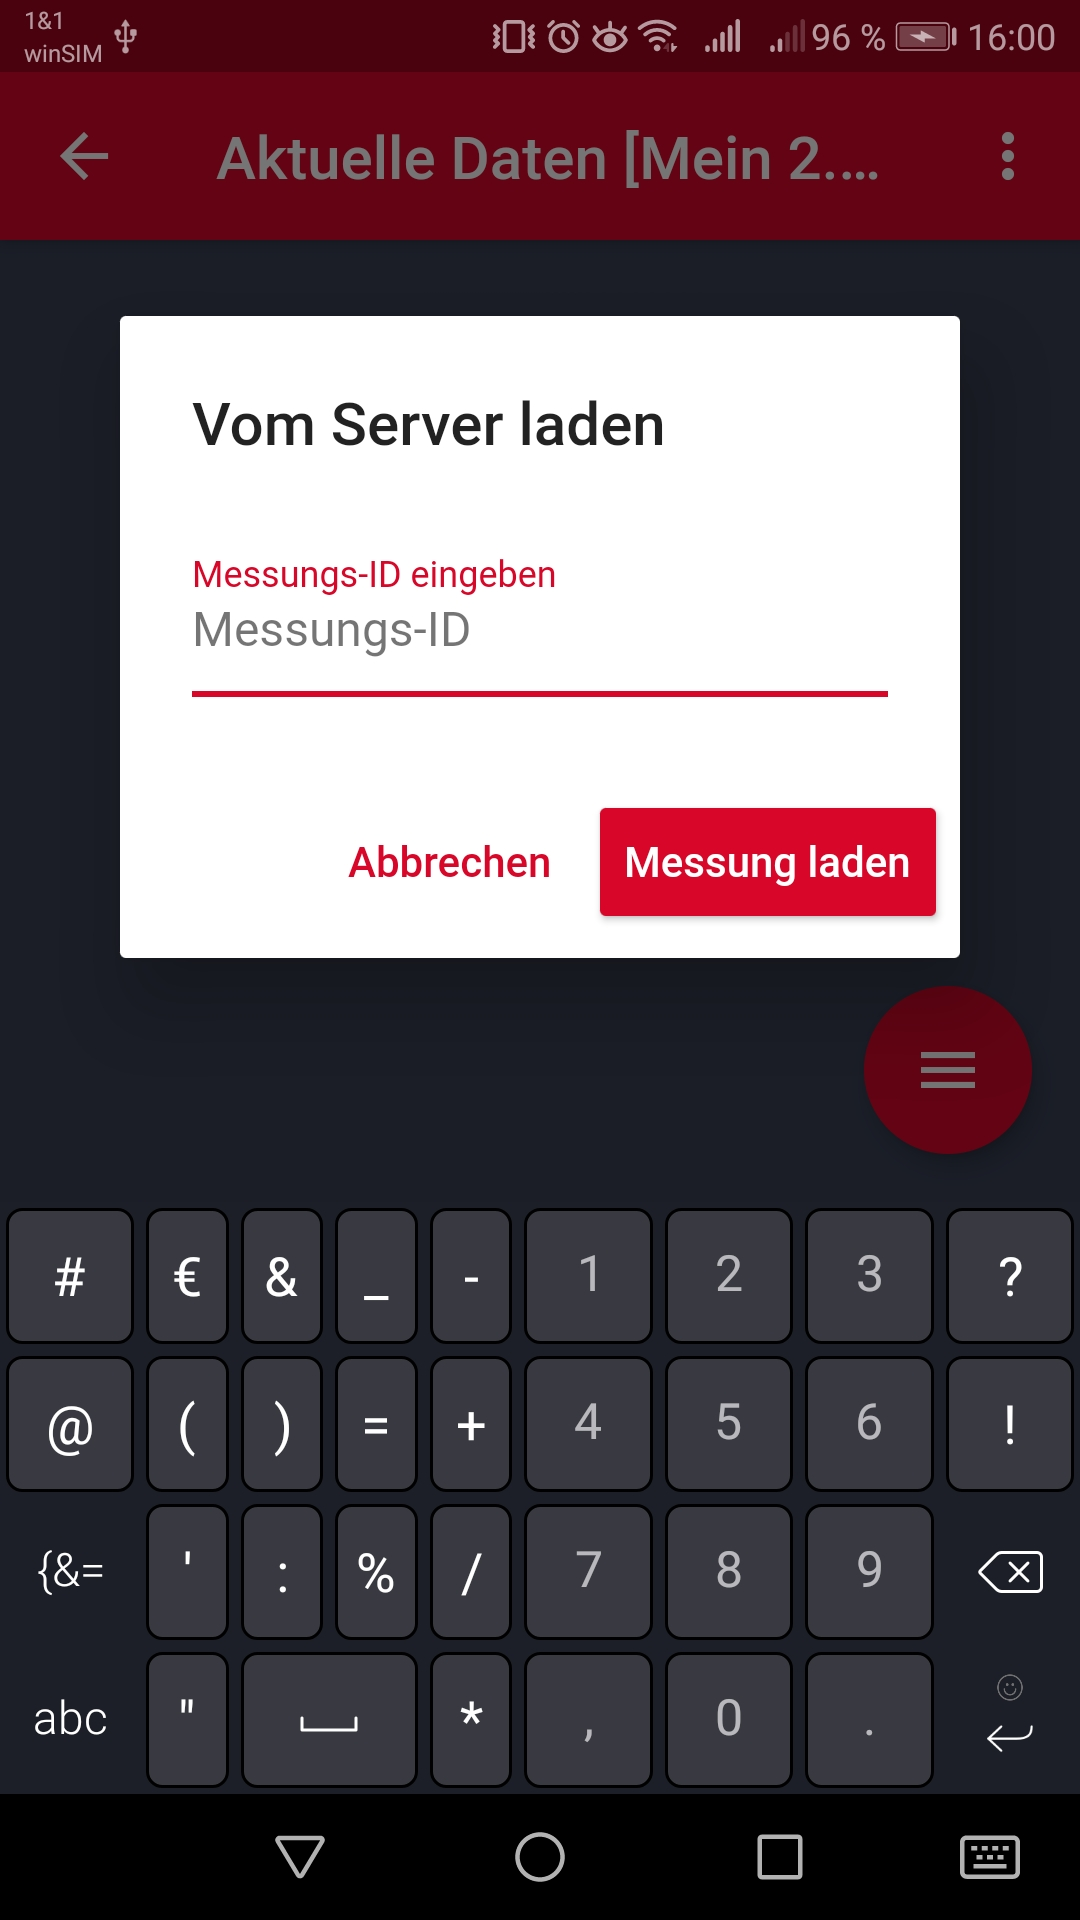
\includegraphics[width=0.6\textwidth]{../include/images/funktionalitaet/dataLaden_fromServer}
		\subcaption{Daten vom Server laden}
	\end{subfigure}
	\hfill
	\begin{subfigure}[b]{0.5\textwidth}
	\centering
		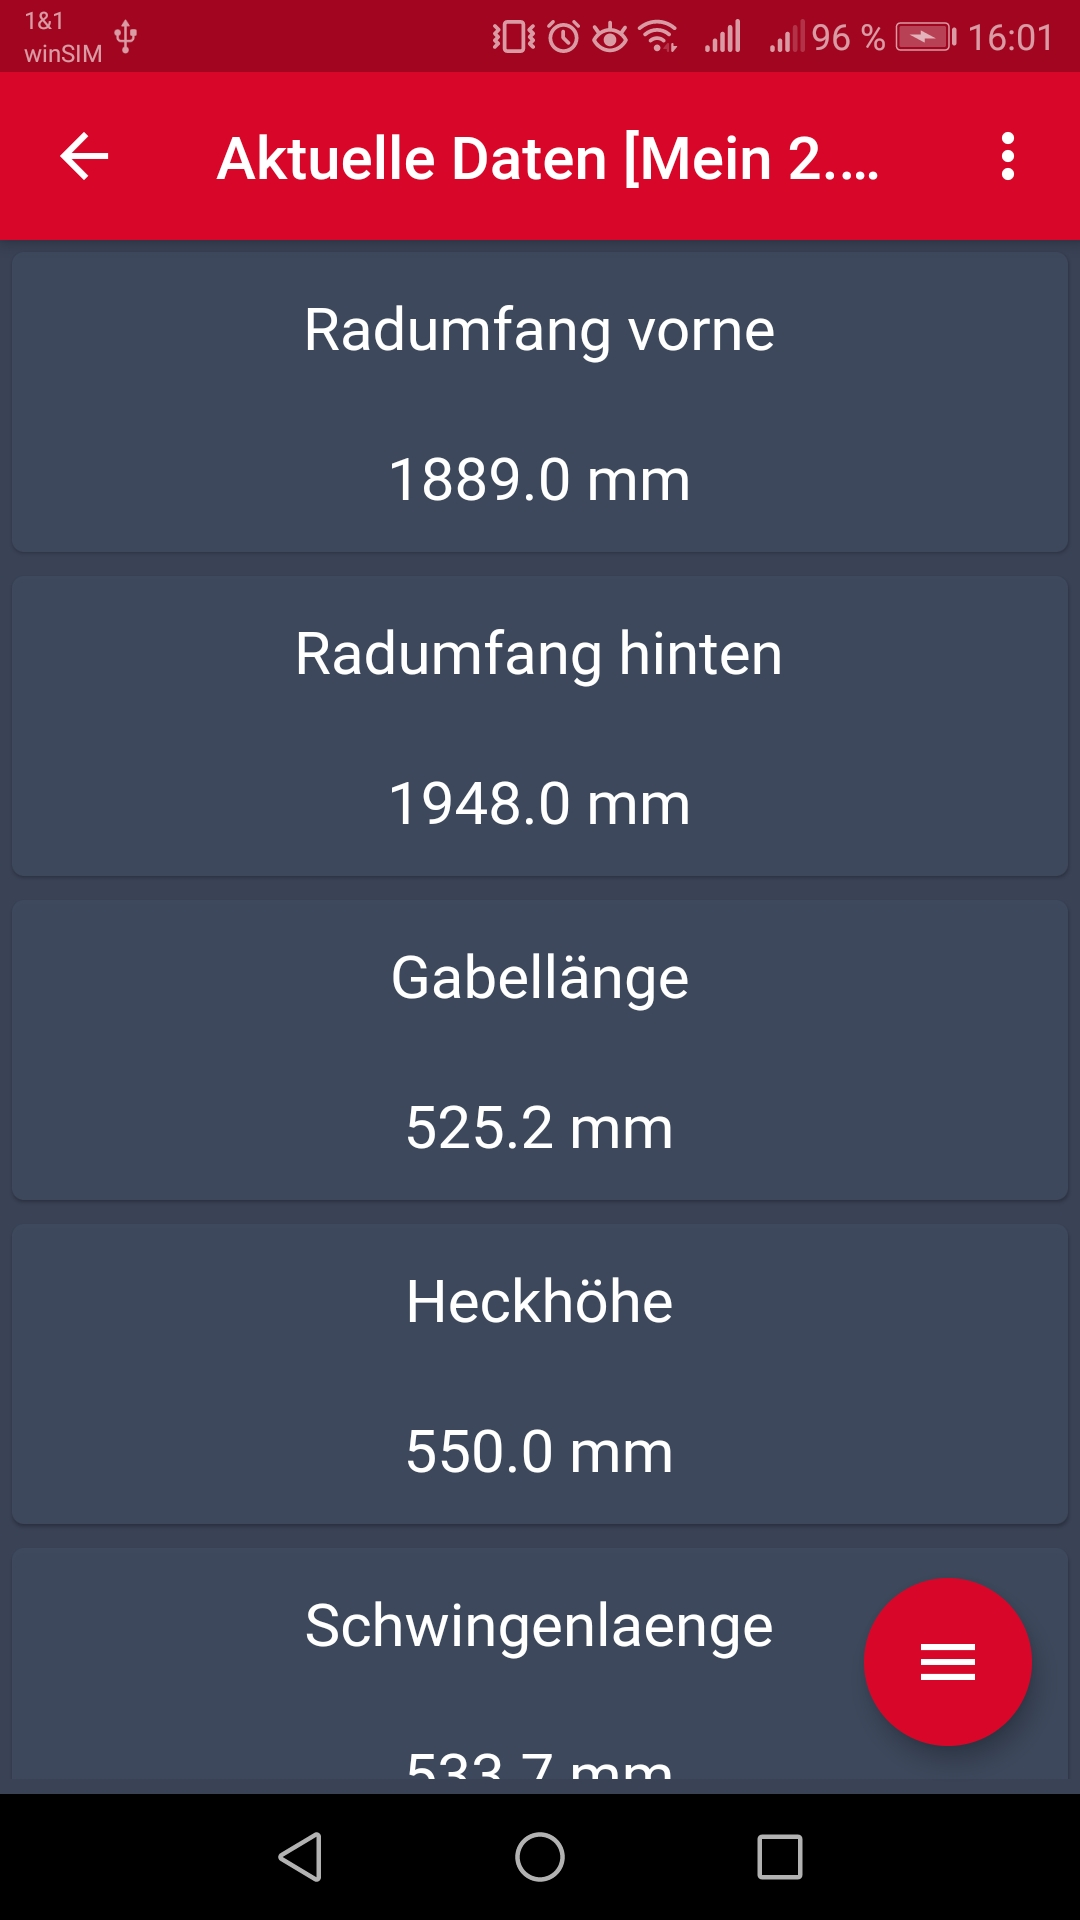
\includegraphics[width=0.6\textwidth]{../include/images/funktionalitaet/dataLaden_withData}
		\subcaption{Nach Laden der Daten}
	\end{subfigure}
	\caption{Die Laden Daten Ansicht}
\end{figure}
		\subsection{Laden aus QR-Code}
		\label{subsec:load-qr}
		Wird der Button \glqq Aus QR-Code laden\grqq{} gedrückt, so öffnet sich die Kamera zum Scannen eines QR-Codes. Sobald der QR-Code erfasst wird, werden die Daten geladen und angezeigt. Ist der QR-Code wiederum ungültig, wird ein Fehler in Form einer Snackbar angezeigt.

	\section{Daten bearbeiten}
	
	Um eine Simulation durchzuführen, müssen gewisse Werte steuerbar sein. In der Daten bearbeiten Ansicht, werden die Kennzahlen dargestellt, die für die Simulation steuerbar sind. Dabei handelt es sich um folgende Kennzahlen:
	
Diese werden in einer Liste dargestellt. Zu jeder Kennzahl werden je drei Werte angezeigt. Links ist der alte Wert und in der Mitte der neue Wert der Kennzahl angezeigt. Auf der rechten Seite sieht man die Differenz zwischen dem neuen und den alten Wert. Ist die Differenz positiv, so wird sie grün, ist sie negativ so wird sie rot dargestellt.
Über Slider oder wahlweise auch Inputfelder kann der neue Wert je Kennzahl verändert werden. Die Einstellung welche Eingabevariante man nutzten möchte, kann in den Einstellungen umgestellt werden.
	\label{sec:edit-data}
	\begin{figure}[H]
	\begin{subfigure}[b]{0.5\textwidth}
		\centering
		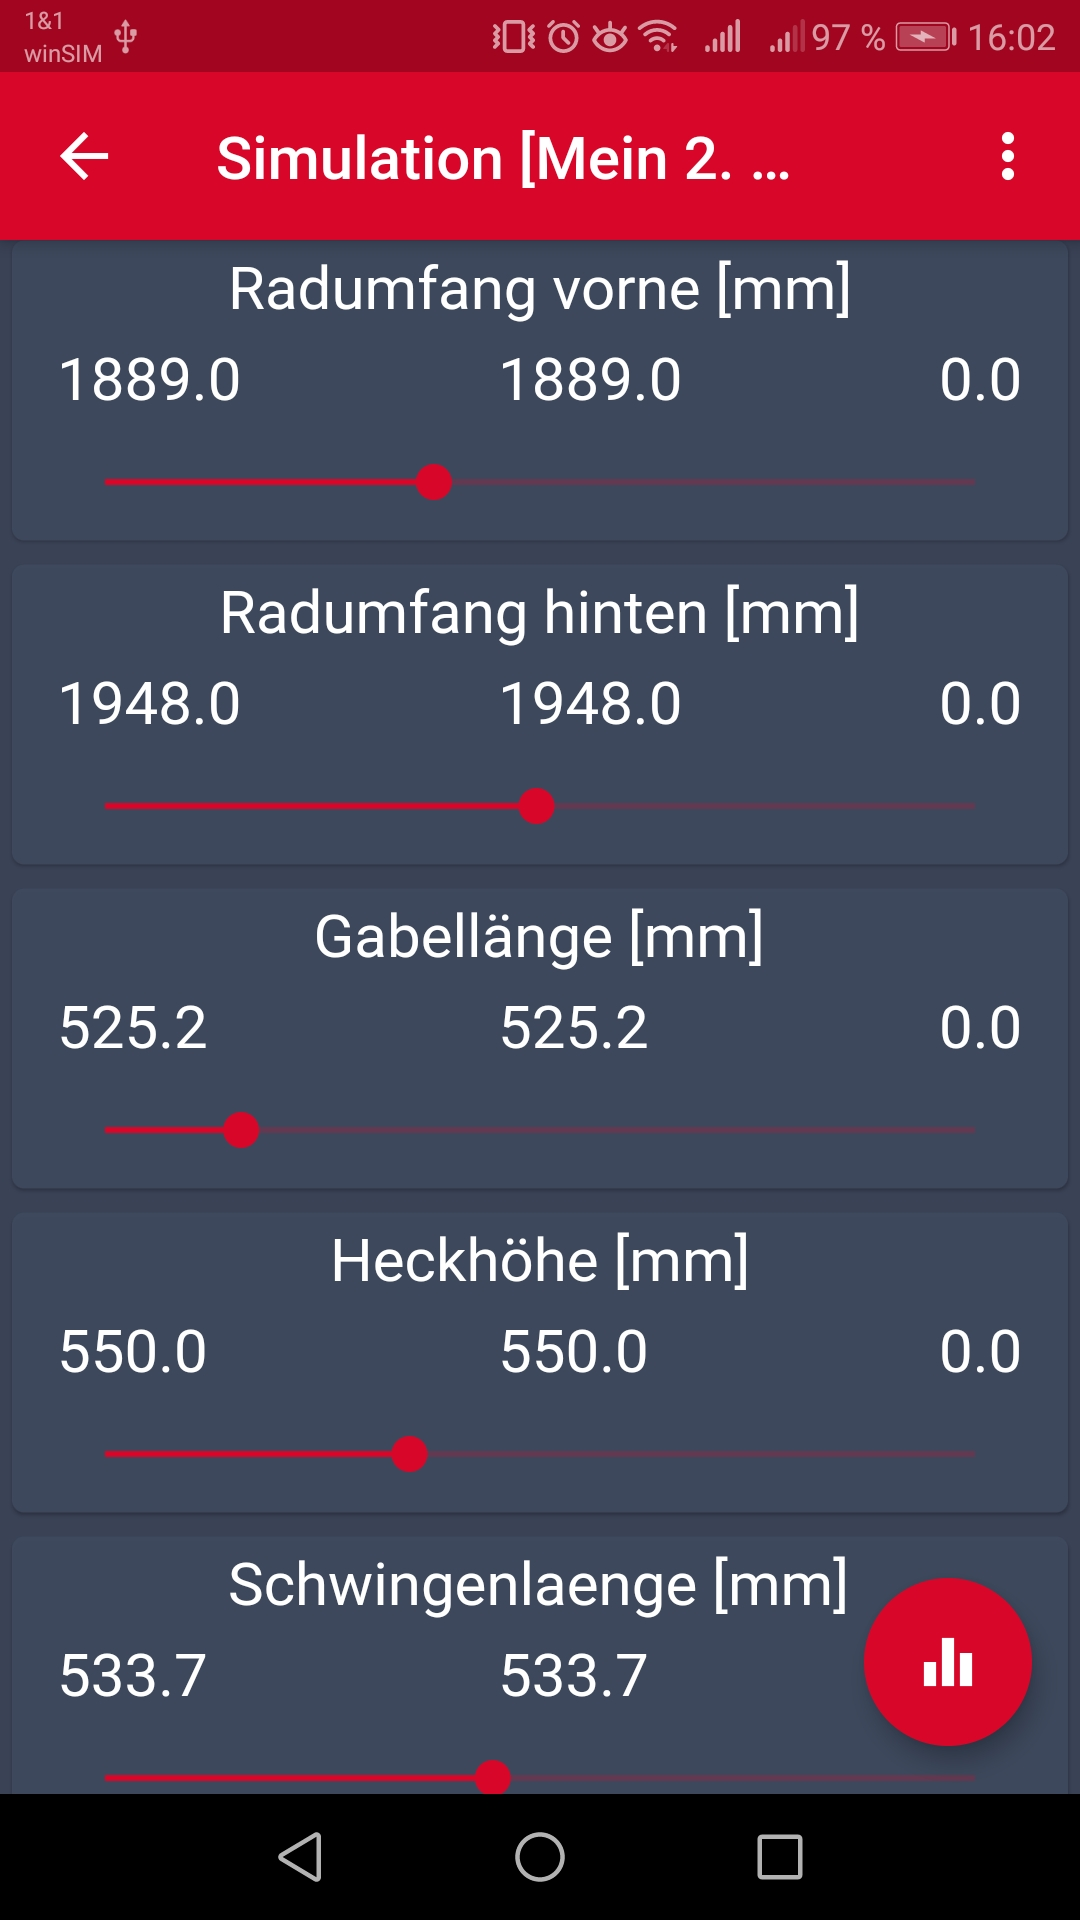
\includegraphics[width=0.6\textwidth]{../include/images/funktionalitaet/dataBearbeiten}
		\subcaption{Mit Slidern}
	\end{subfigure}
	\hfill
	\begin{subfigure}[b]{0.5\textwidth}
	\centering
		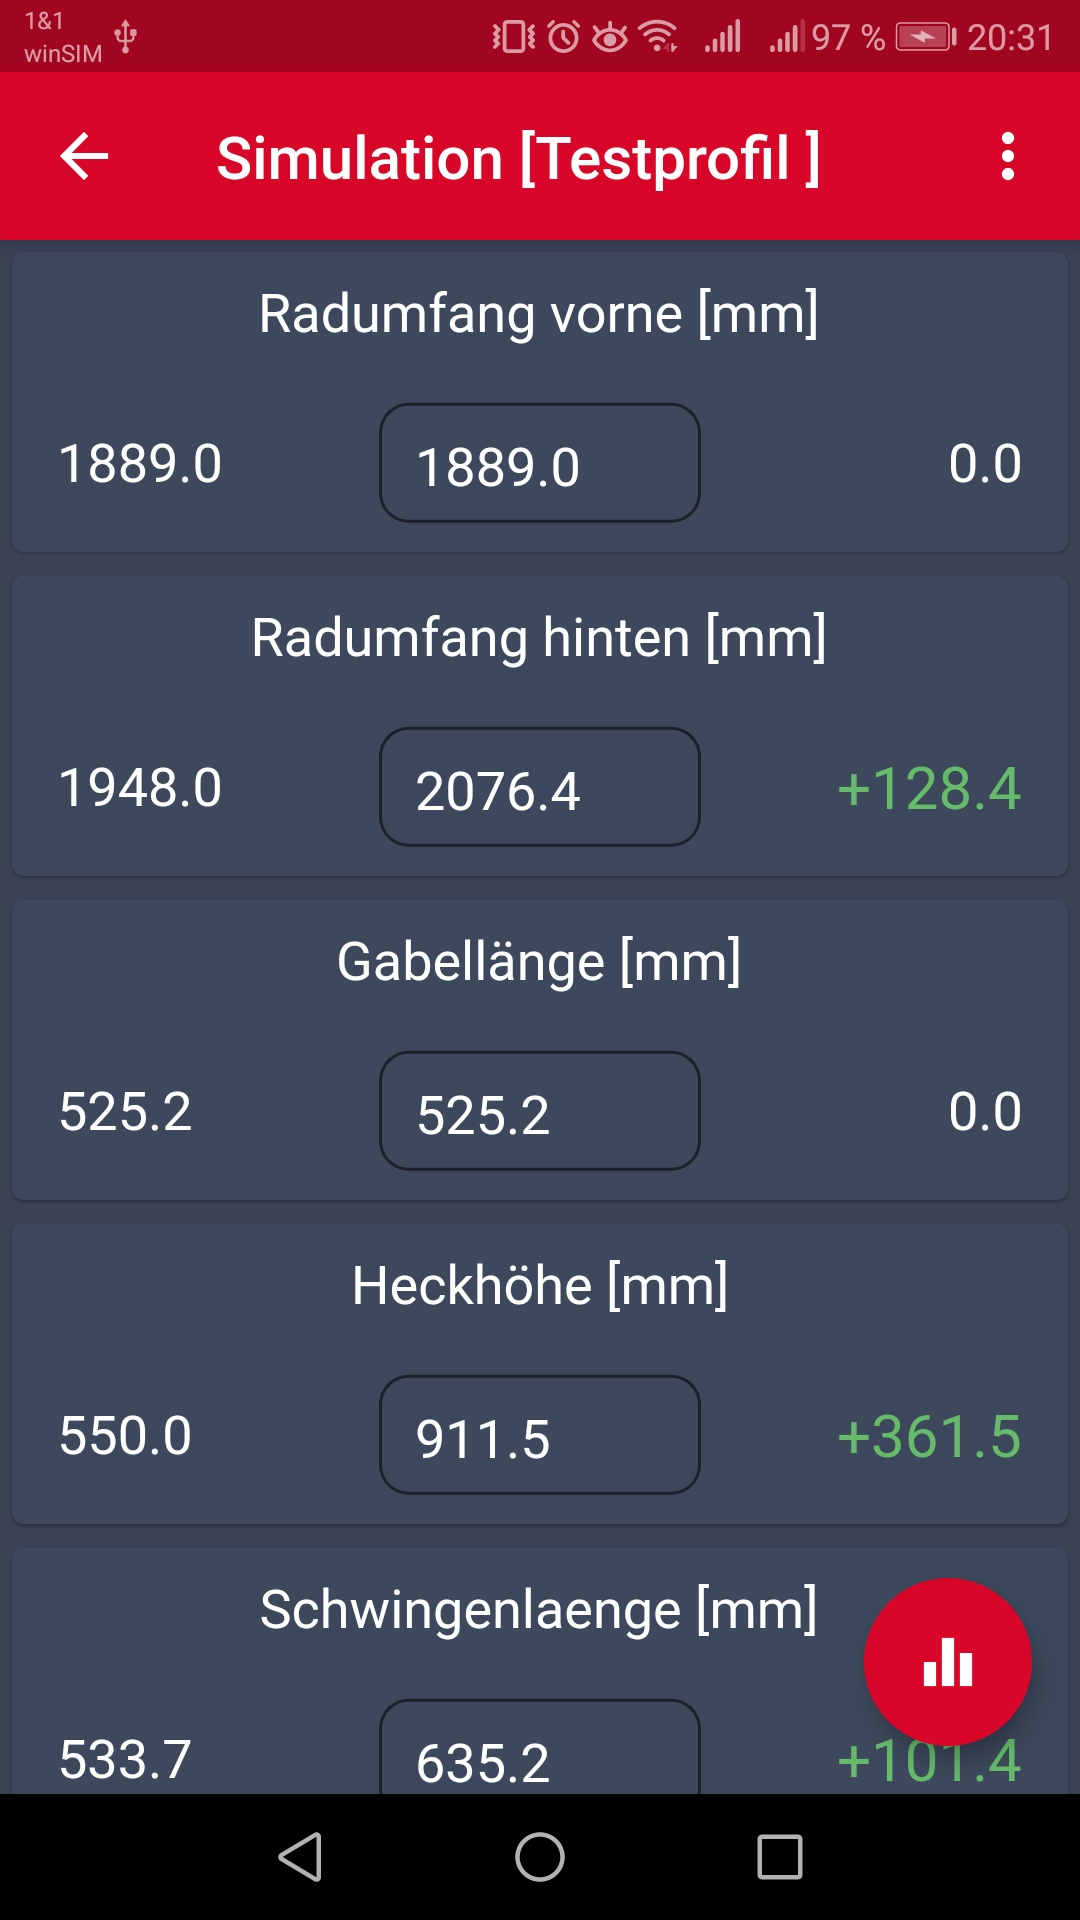
\includegraphics[width=0.6\textwidth]{../include/images/funktionalitaet/dataBearbeitenInput}
		\subcaption{Als Inputfeld}
	\end{subfigure}		
	
	\caption{Daten bearbeiten Ansicht}
\end{figure}
	
	
	\section{Simulation}
	\label{sec:sim}
	
	Die Simulation wird auf einer Seite mit drei Tabs dargestellt.  Der Tab in der Mitte beinhaltet Diagramme. Dieser wird standardmäßig als erstes geöffnet. Durch eine Wischbewegung (swipen) nach links oder rechts, kann man auf die anderen Tabs gelangen. Der Tab auf der linken Seite stellt die Ergebnisse als Tabelle dar. Zusammen mit dem Diagramm-Tab werden dort die Ergebnisse der Simulation angezeigt. Der Tab auf der rechten Seite hingegen, ist nur um zusätzliche Informationen zur Simulation hinzuzufügen.
	
		\subsection{Diagramme}
		\label{subsec:diagr}
		
		Der Diagrammtab beinhaltet fünf Diagramme. Das erste Diagramm ist ein Balkendiagramm, das eine Übersicht über die Veränderungen geben soll. Es stellt die größten prozentuellen Veränderungen der Kennzahl dar. Dies bietet dem User die Möglichkeit auf einem Blick zu sehen, welche Kennzahlen sich am meisten verändert haben. Zur Vergleichbarkeit zwischen Winkeln und Längenmaßen wurde wird hier die prozentuelle Veränderung angezeigt. Kennzahlen, die durch die Simulattion kleiner werden, werden durch rote Balken gekennzeichnet. Sich vergrößernde Kennzahlen hingegen werden grün dargestellt. Gleiches gilt auch für die vier folgenden Diagramme. Die Single Kennzahl Diagramme, zeigen die Veränderung einer Kennzahl im Detail an. Dabei werden der alte und neuer Wert, sowie die Differenz angezeigt. Zusätzlich wird anhand eines Säulendiagramms der alte und neue Wert der Kennzahl nochmal grafisch dargestellt. Single Kennzahl Diagramme werden für die vier Kennzahlen mit der größten absoluten Änderung dargestellt.
		
		
	\begin{figure}[H]
	\begin{subfigure}[b]{0.5\textwidth}
		\centering
		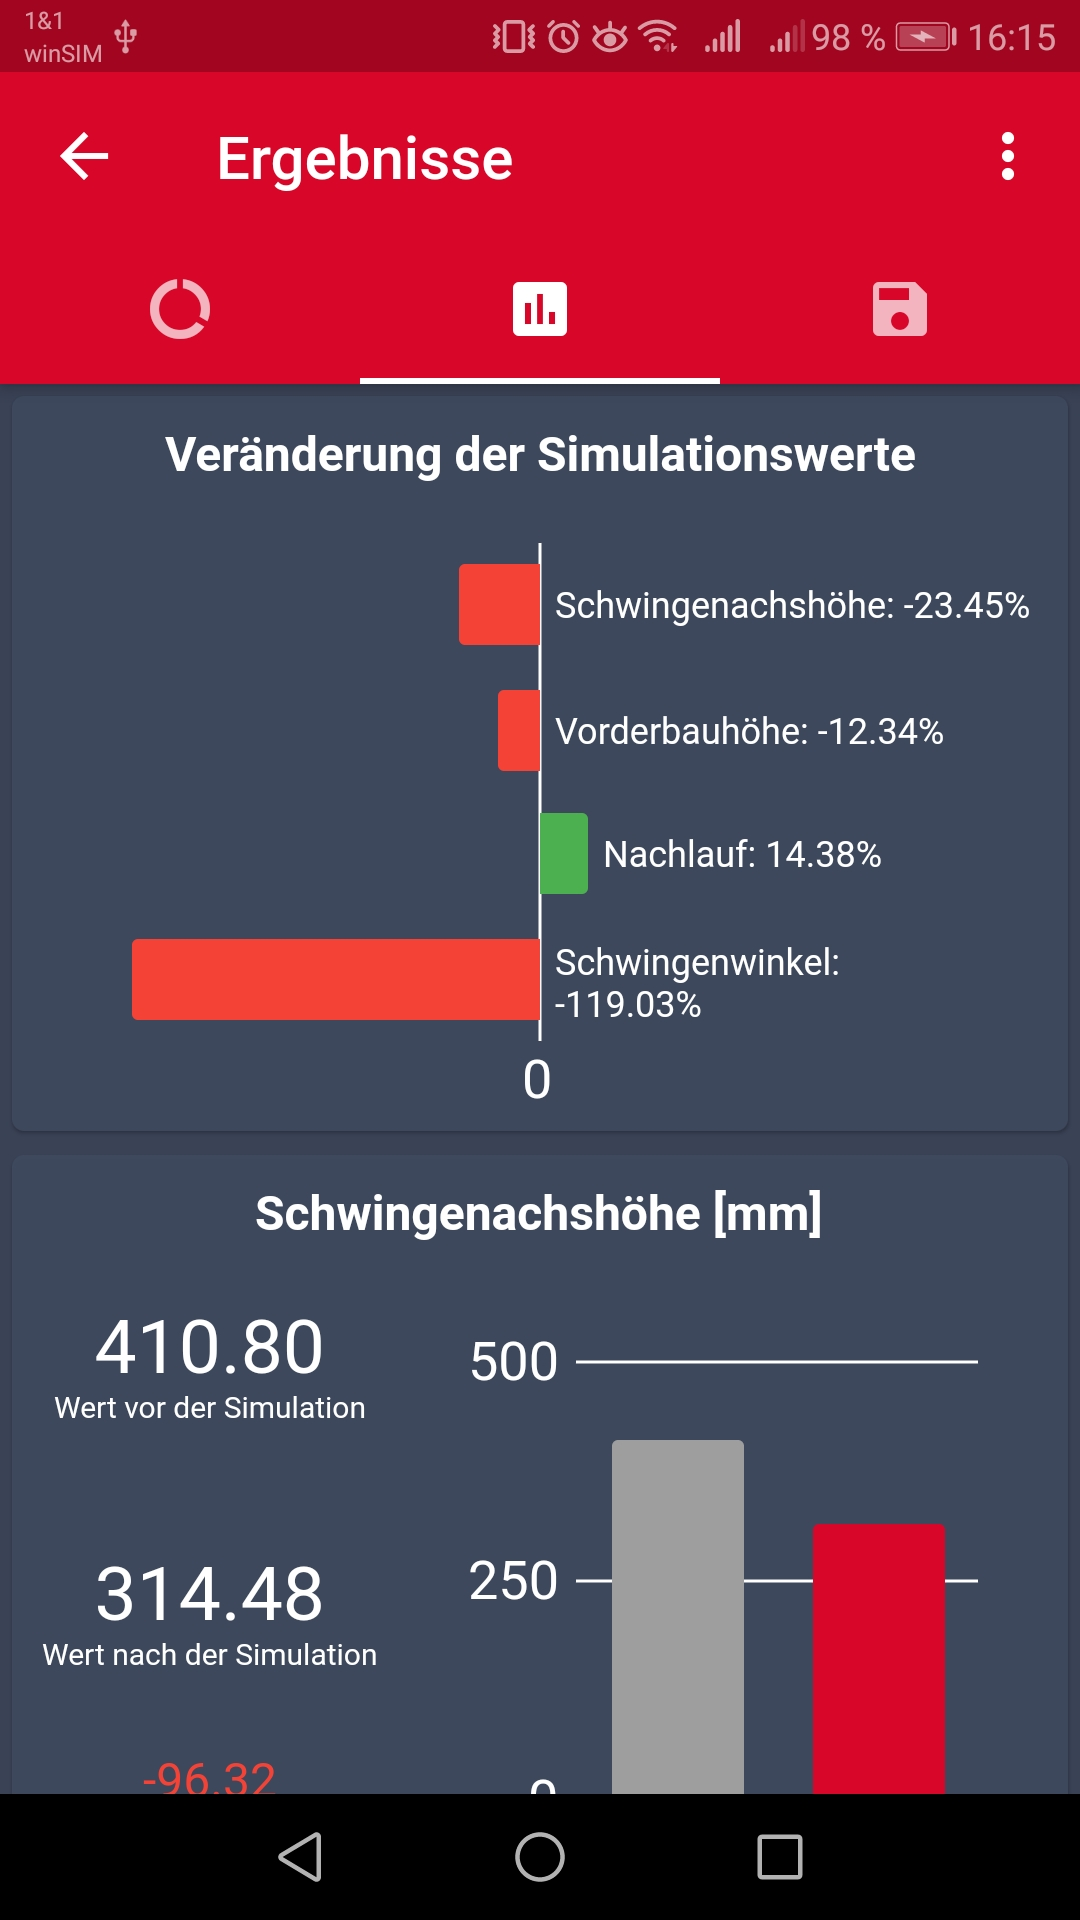
\includegraphics[width=0.6\textwidth]{../include/images/funktionalitaet/diagramm_1}
		\subcaption{Übersichtsdiagramm}
	\end{subfigure}
	\hfill
	\begin{subfigure}[b]{0.5\textwidth}
	\centering
		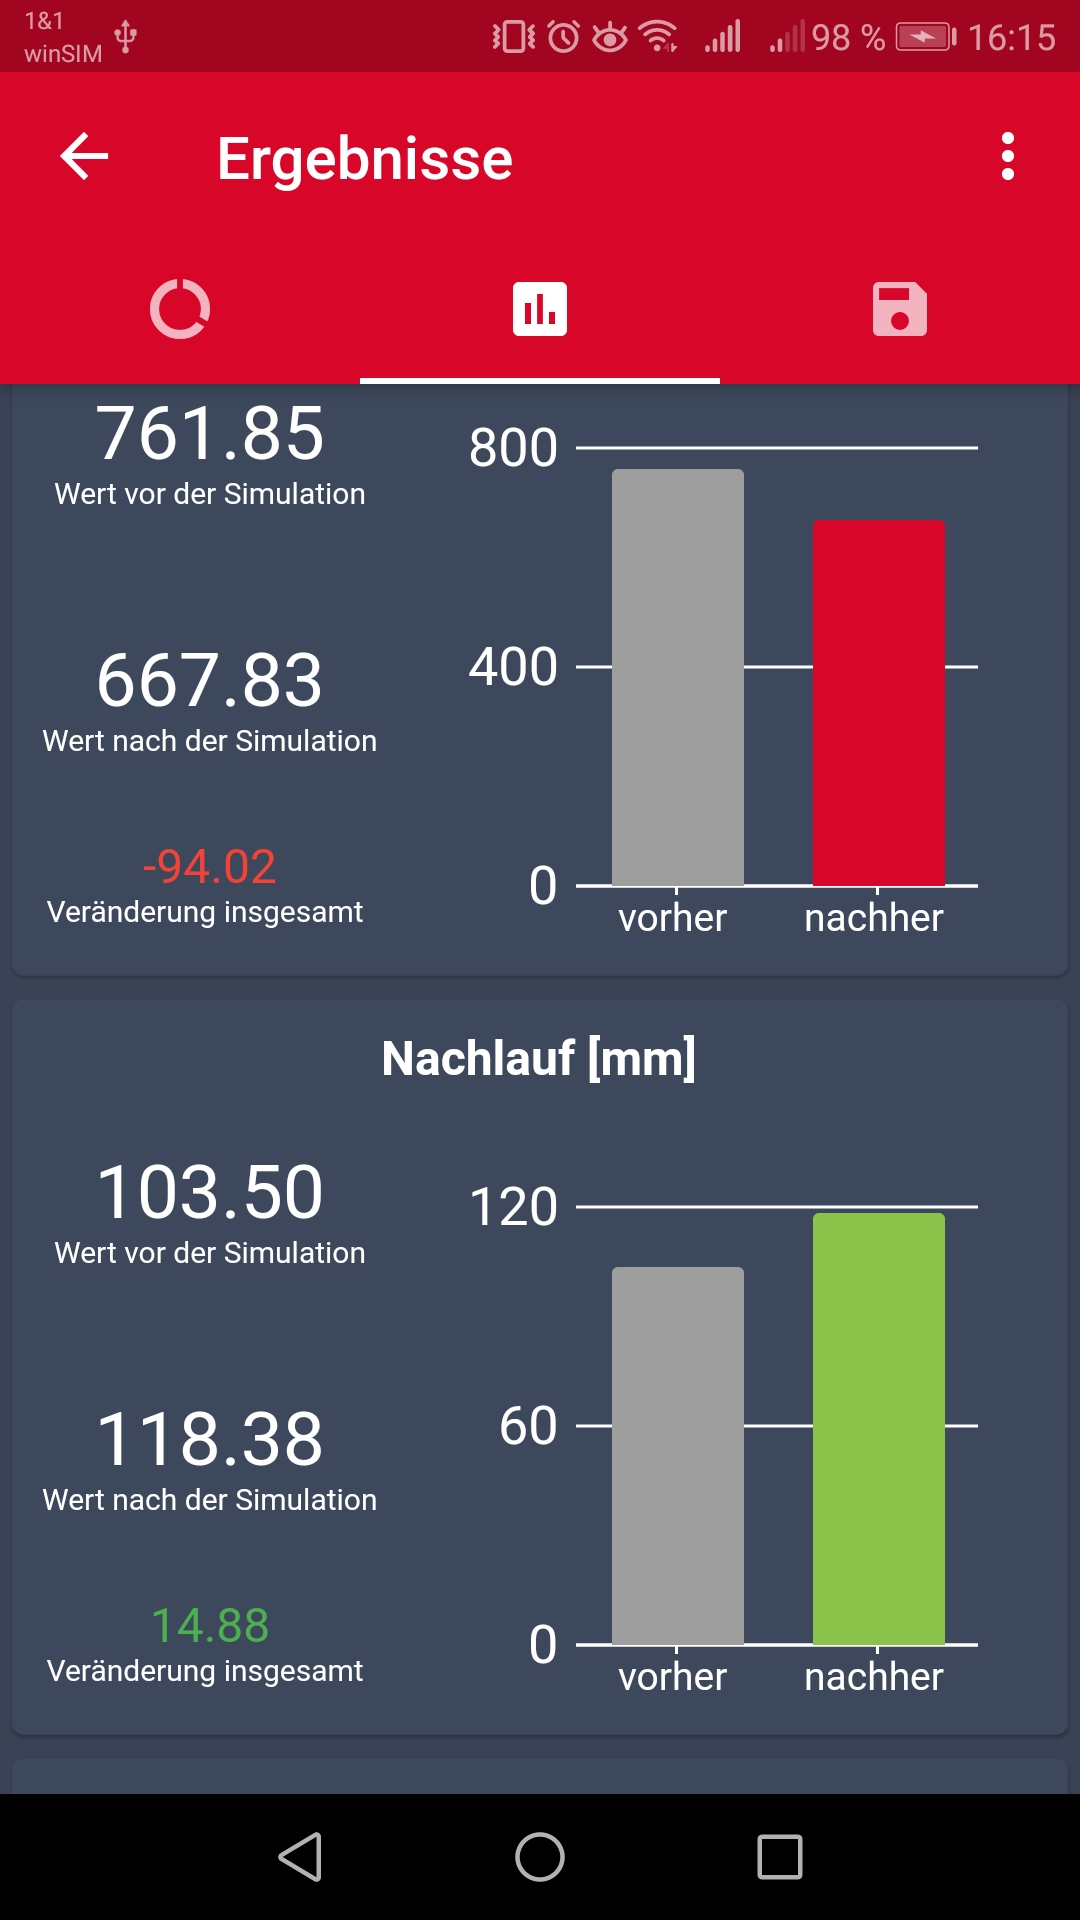
\includegraphics[width=0.6\textwidth]{../include/images/funktionalitaet/diagramm_2}
		\subcaption{Single Kennzahl Diagramm}
	\end{subfigure}		
	
	\caption{Diagrammtypen}
\end{figure}
		
		
		\subsection{Tabelle}
		\label{subsec:table}
		Die Tabellenansicht gibt einen guten Überblick über die alle Werte an. Dabei werden zunächst die aus der Simulation hervorgehenden Werte angezeigt. Anschließend werden die bearbeiteten Eingabewerte angezeigt. So kann der Nutzer erkennen aus welchen Eingabewerten, welches Simulationsergebnis vorher geht. Es werden, wie auch in der Dateneingabe der alte und neue Wert der Kennzahl, sowie die Differenz angezeigt.
		
	\begin{figure}[H]
	\begin{subfigure}[b]{0.5\textwidth}
		\centering
		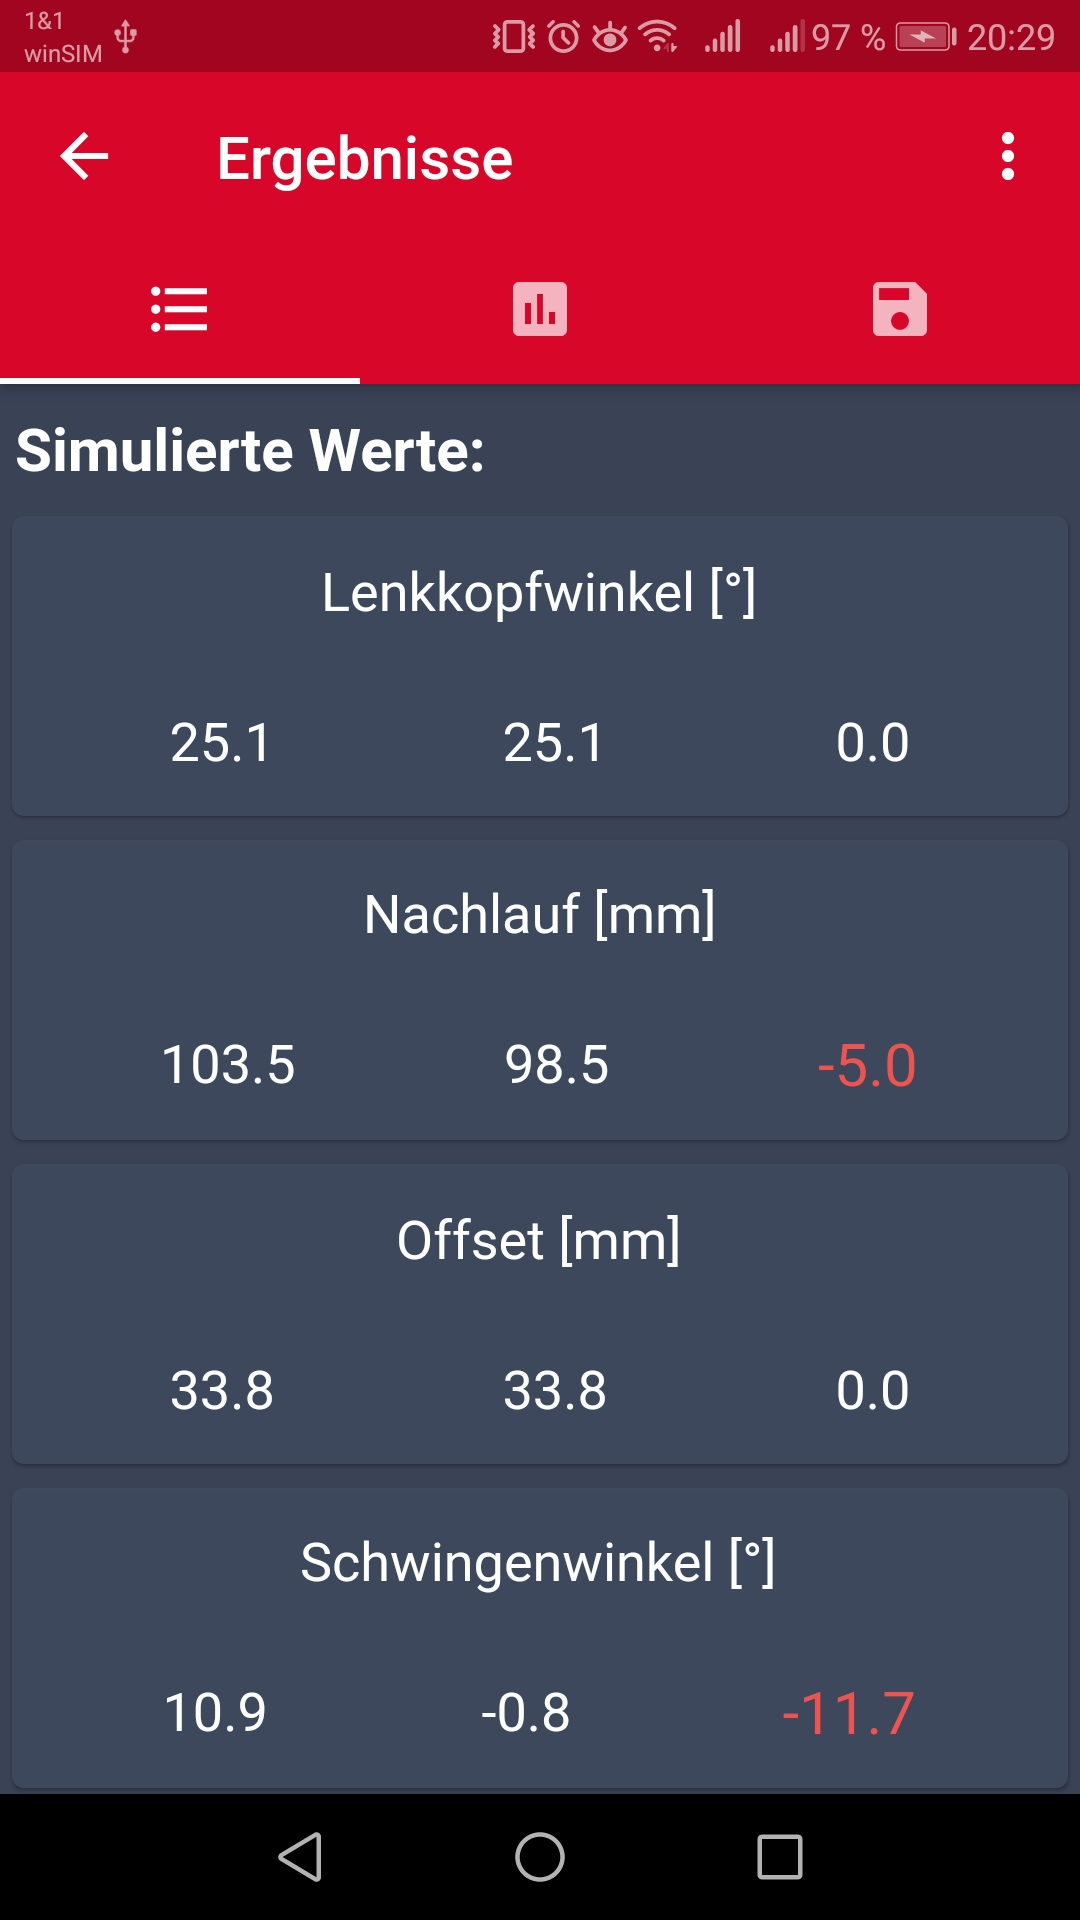
\includegraphics[width=0.6\textwidth]{../include/images/funktionalitaet/simval}
		\subcaption{Simulationswerte}
	\end{subfigure}
	\hfill
	\begin{subfigure}[b]{0.5\textwidth}
	\centering
		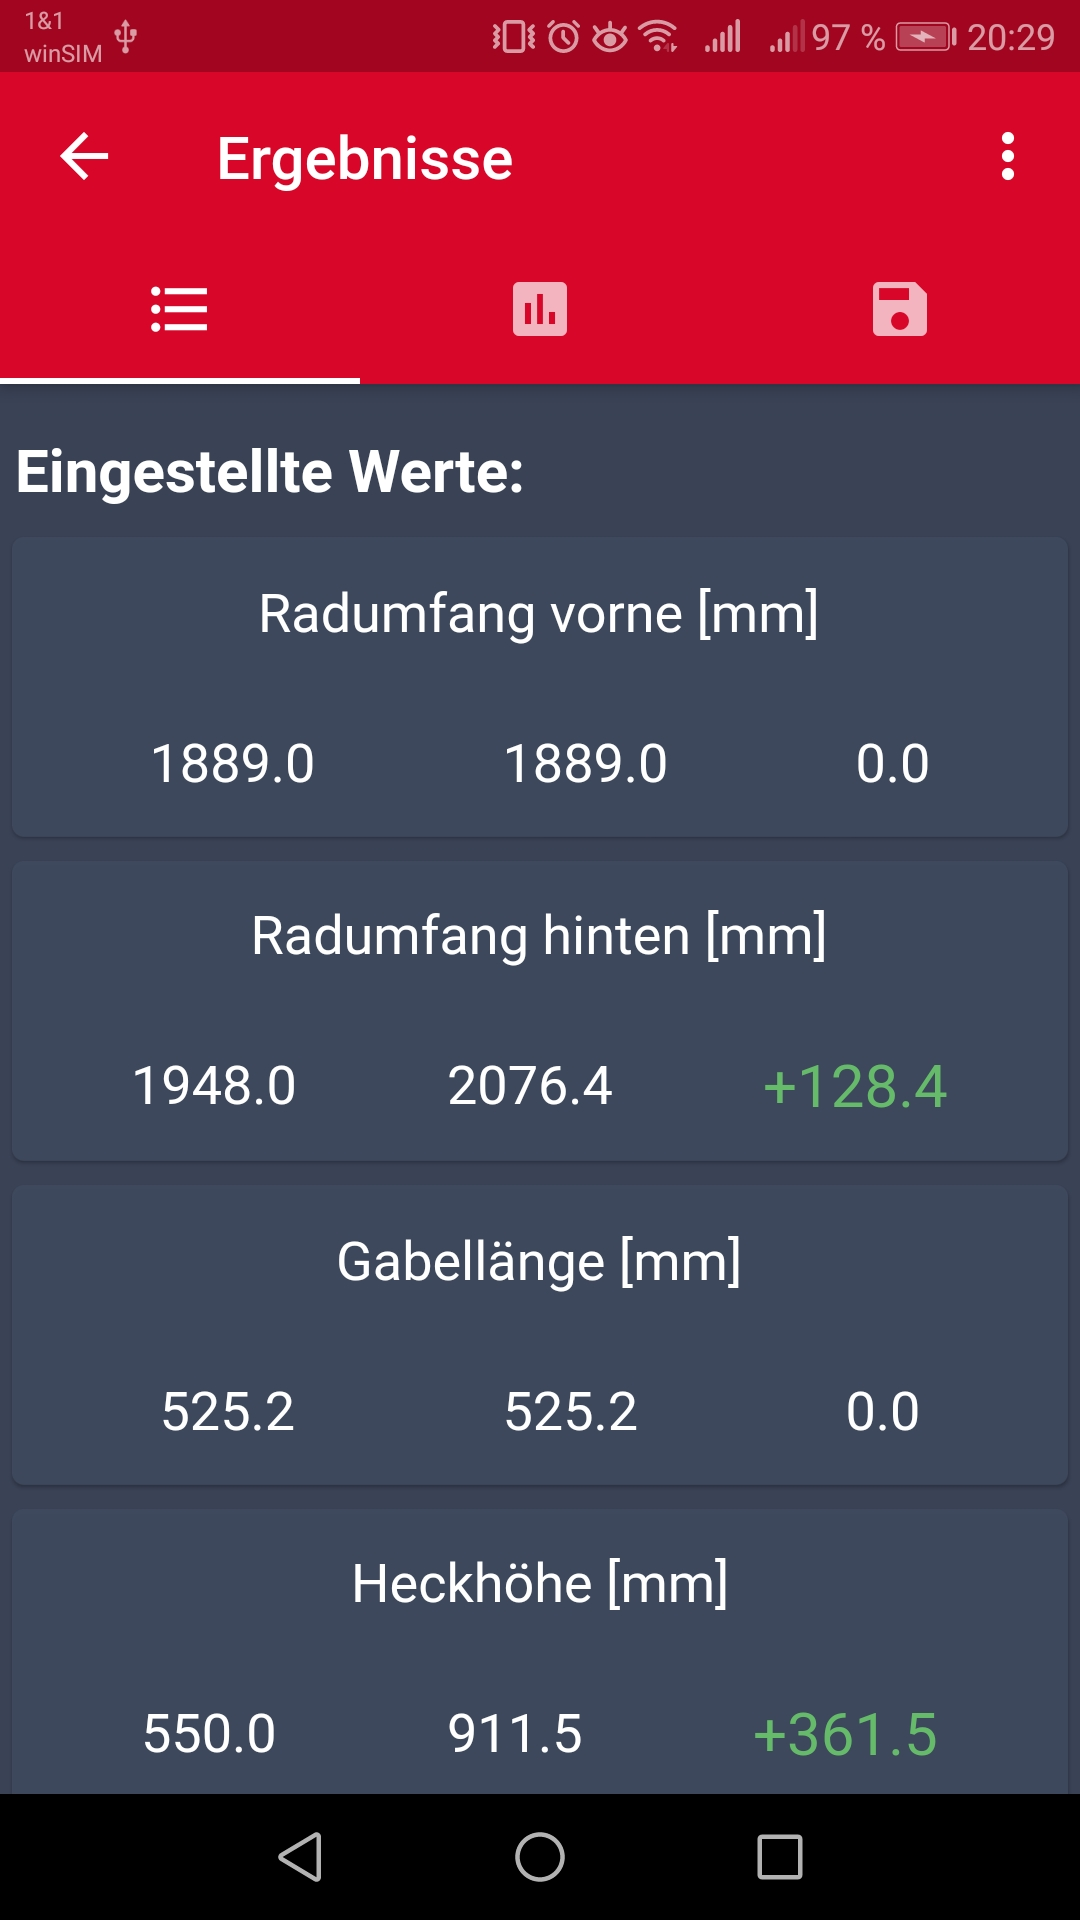
\includegraphics[width=0.6\textwidth]{../include/images/funktionalitaet/einval}
		\subcaption{Eingabewerte}
	\end{subfigure}		
	
	\caption{Daten bearbeiten Ansicht}
\end{figure}
		\subsection{Kommentar}
		\label{subsec:comment}
		Die Kommentarseite bietet dem User die Möglichkeit eine Notiz oder einen Kommentar für die Simulation zu speichern. Ein Textfeld ermöglicht die Eingabe des Kommentars. Der Kommentar wird dabei automatisch gespeichert.
	\begin{figure}[H]
	\centering
		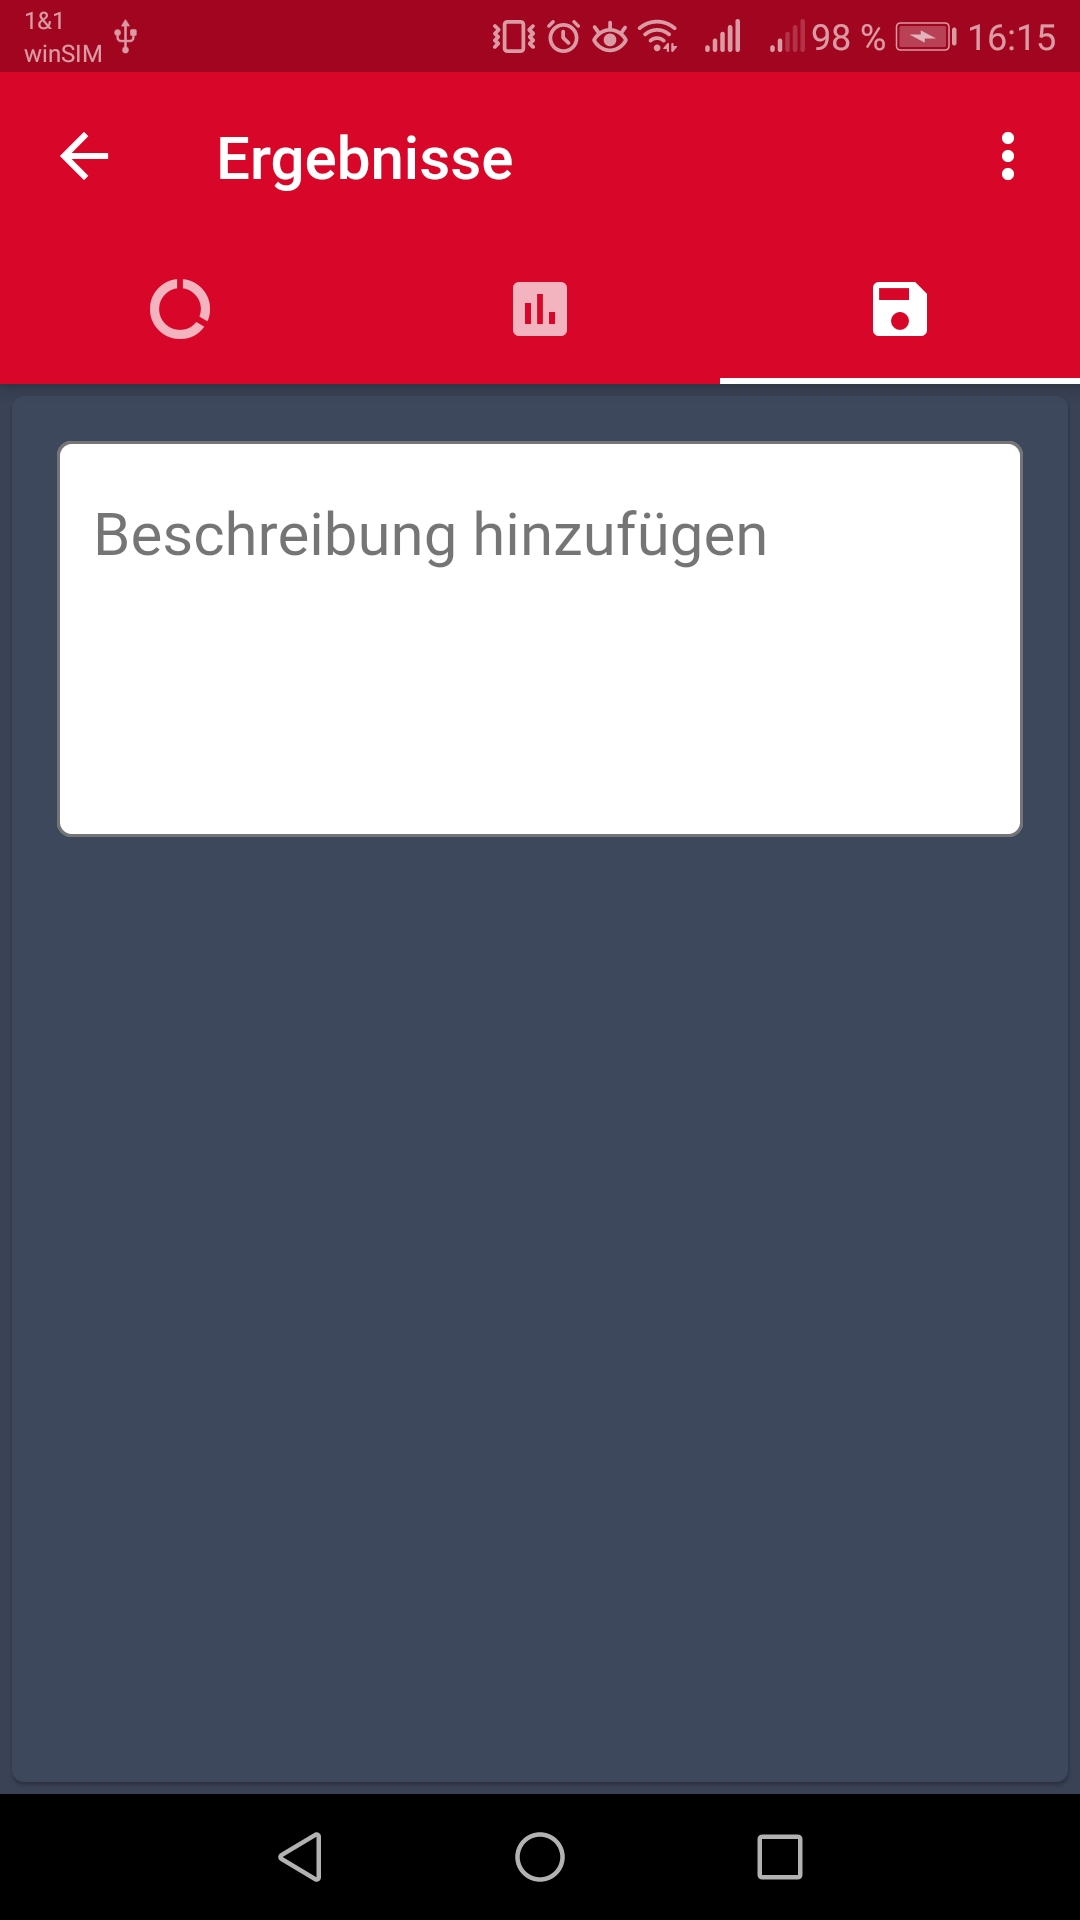
\includegraphics[width=0.3\textwidth]{../include/images/funktionalitaet/Kommentar}
	
	\caption{Kommentarseite}
\end{figure}
	
	
		